% Preamble
\documentclass[12pt,a4paper]{article}
\usepackage{enumerate} 	
\usepackage{setspace}						
\usepackage{authblk}	
\usepackage{graphicx} 	
%\usepackage[nomarkers, nolists]{endfloat} 
\usepackage{pdflscape}	
\usepackage{mathtools}	
\usepackage[osf]{mathpazo} 
\usepackage{lineno} 
\usepackage{ms}    	
\usepackage{hyperref}
\usepackage[round]{natbib} 
\usepackage{setspace}

\setcounter{secnumdepth}{0} 
\raggedright 			
\pagenumbering{arabic}	
\linenumbers


% First order headings upper case bold
\usepackage{titlesec}
\titleformat*{\section}{\small\bfseries\uppercase}

% Second order headings normal case italics
\titleformat*{\subsection}{\small\itshape}

% Third order, italics, paragraph style
\titleformat*{\paragraph}{\small\itshape}


% lists - arabic in (1; (2); (3) .


% Title page information

\title{Supporting Information from `Time for a rethink: time sub-sampling methods in disparity-through-time analyses'}

\author{
	Thomas Guillerme$^{1*}$ and Natalie Cooper$^{2}$
}

\date{}

\affiliation{\noindent{\footnotesize
	$^1$School of Biological Sciences, University of Queensland, St. Lucia, Queensland, Australia.\\
	$^2$Department of Life Sciences, Natural History Museum, Cromwell Road, London, SW7 5BD, UK. natalie.cooper@nhm.ac.uk}\\
	$^*$Corresponding author\\}

\vfill

%\runninghead{Time sub-samples in disparity-through-time analyses}
%\keywords{time bin, time slice, disparity} 
% up to 6

\begin{document}

\mstitlepage
\parindent = 1.5em
\addtolength{\parskip}{.3em}

%\section{Abstract}
% 300 words max
	

\newpage
\raggedright
\doublespacing
\setlength{\parindent}{1cm}

\section{Additional tables and figures}

  \begin{figure}[!htbp]
    \centering
    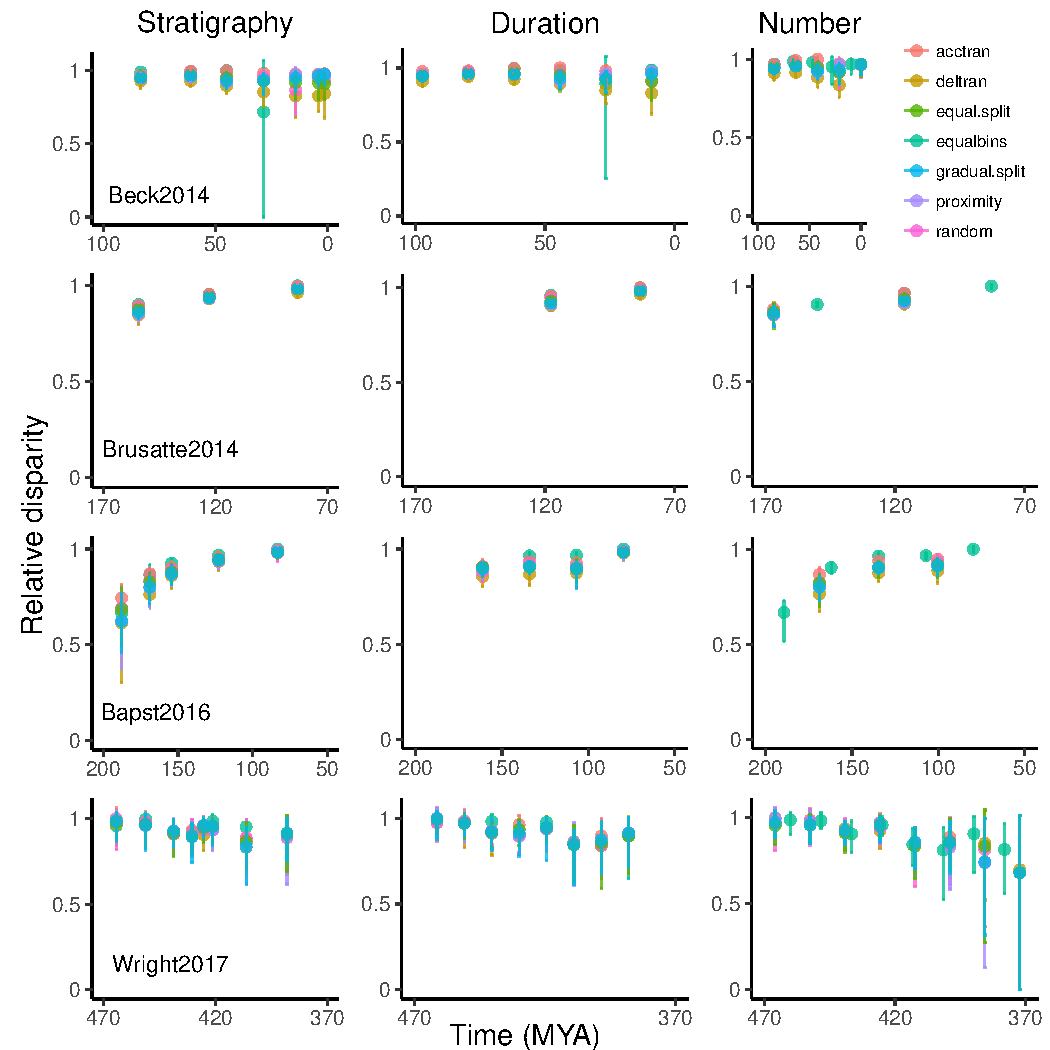
\includegraphics[width=1\linewidth, height=1\textheight, keepaspectratio]{figures/fig-dtt-epoch-appendix.pdf}
    \caption[Relative disparity through time for four example datasets.]
    {Median bootstrapped disparities were calculated using time binning and time-slicing approaches. 
    Pink points represent time binning methods, 
    % blue points are time slices with a punctuated model of evolution (specifically the `proximity' method), and green points are time slices with a gradual model of evolution (specifically the `gradual splits' method).
    Relative disparities (median bootstrapped disparity divided by the maximum median bootstrapped disparity for a dataset and analysis method) are presented so they can be compared across datasets/methods. 
    Stratigraphy uses unequal time bins or non-equidistant slices, where the width of the bin, or the interval between slices, is equivalent to stratigraphic epochs. 
    Duration uses equal time bins or equidistant slices, where the width of the bin, or the interval between slices, is the average duration of stratigraphic epochs in the time frame of the dataset. 
    Number uses equal time bins or equidistant slices, where the number of bins, or the number of slices, is the average number of stratigraphic epochs in the time frame of the dataset. 
    In all cases, time bin disparities are plotted at the midpoint of the bin, and error bars represent the 95\% confidence intervals around the bootstrapped median disparity.
    The four dataset names are on the first plot for each dataset (Table \ref{table:datasets}).}
    \label{figure:dtt2}
  \end{figure}  

  \begin{figure}[!htbp]
    \centering
    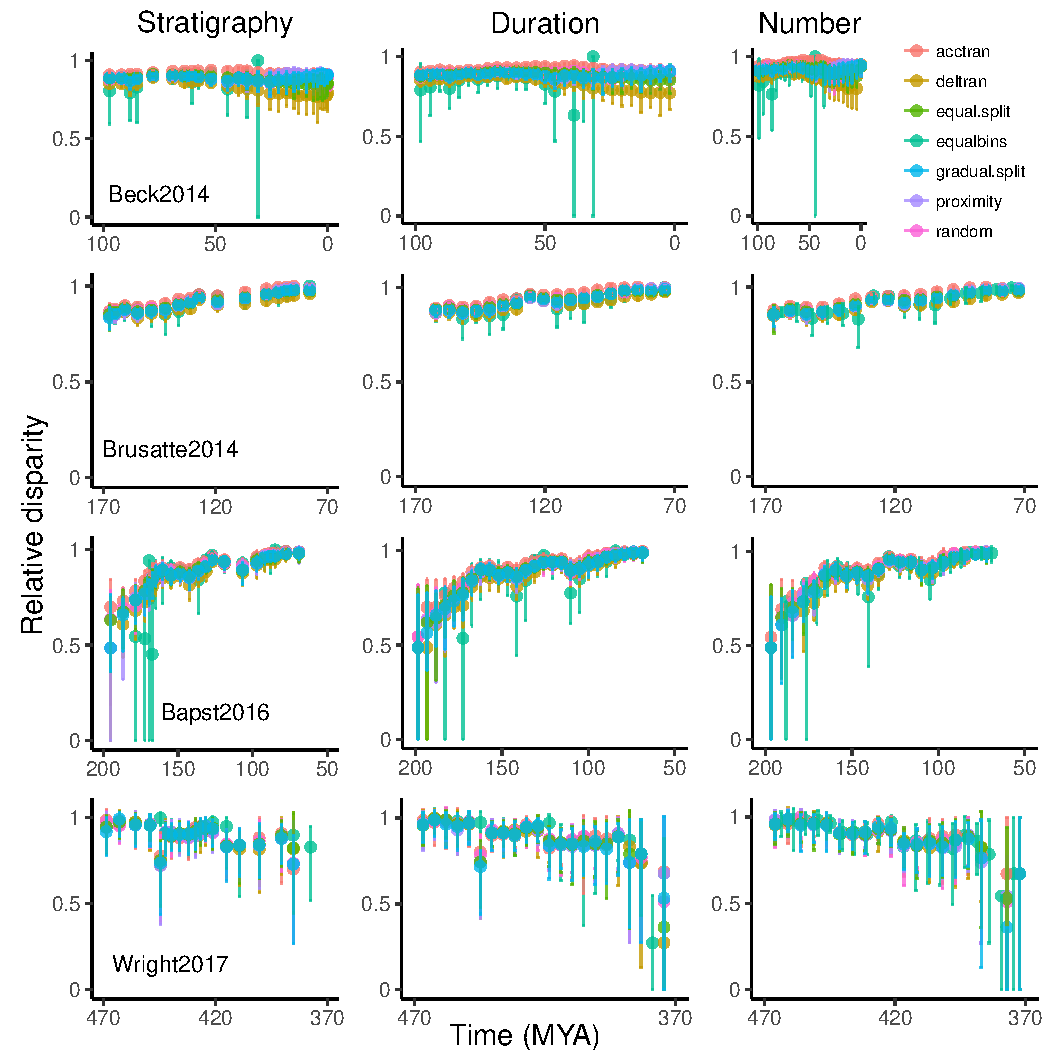
\includegraphics[width=1\linewidth, height=1\textheight, keepaspectratio]{figures/fig-dtt-age-appendix.pdf}
    \caption[Relative disparity through time for four example datasets.]
    {Median bootstrapped disparities were calculated using time binning and time-slicing approaches. 
    Pink points represent time binning methods, 
    %blue points are time slices with a punctuated model of evolution (specifically the `proximity' method), and green points are time slices with a gradual model of evolution (specifically the `gradual splits' method).
    Relative disparities (median bootstrapped disparity divided by the maximum median bootstrapped disparity for a dataset and analysis method) are presented so they can be compared across datasets/methods. 
    Stratigraphy uses unequal time bins or non-equidistant slices, where the width of the bin, or the interval between slices, is equivalent to stratigraphic ages. 
    Duration uses equal time bins or equidistant slices, where the width of the bin, or the interval between slices, is the average duration of stratigraphic ages in the time frame of the dataset. 
    Number uses equal time bins or equidistant slices, where the number of bins, or the number of slices, is the average number of stratigraphic ages in the time frame of the dataset. 
    In all cases, time bin disparities are plotted at the midpoint of the bin, and error bars represent the 95\% confidence intervals around the bootstrapped median disparity.
    The four dataset names are on the first plot for each dataset (Table \ref{table:datasets}).}
    \label{figure:dtt3}
  \end{figure}  

  % Wilcoxon results table
%\begin{landscape}
  % latex table generated in R 3.4.2 by xtable 1.8-2 package
% Fri Dec  8 17:06:33 2017
\begin{table}[!htbp]
\centering
\begin{tabular}{lllccc}
  \hline
\textbf{Dataset} & \textbf{Period} & \textbf{Model} & \textbf{Stratigraphy} & \textbf{Duration} & \textbf{Number} \\ 
  \hline
Beck2014 & Age & acctran & 39*** & 76 & 11 \\ 
  Beck2014 & Age & deltran & 188*** & 194*** & 171 \\ 
  Beck2014 & Age & equal.split & 91 & 119*** & 47 \\ 
  Beck2014 & Age & gradual.split & 111 & 115*** & 65*** \\ 
  Beck2014 & Age & proximity & 105 & 83 & 68*** \\ 
  Beck2014 & Age & random & 97 & 104*** & 45 \\ 
  Beck2014 & Epoch & acctran & 14 & 10 & 14 \\ 
  Beck2014 & Epoch & deltran & 21 & 45*** & 41*** \\ 
  Beck2014 & Epoch & equal.split & 21 & 40*** & 42*** \\ 
  Beck2014 & Epoch & gradual.split & 21 & 39 & 43*** \\ 
  Beck2014 & Epoch & proximity & 21 & 36 & 32 \\ 
  Beck2014 & Epoch & random & 21 & 37 & 45*** \\ 
  Brusatte2014 & Age & acctran & 27*** & 28 & 28*** \\ 
  Brusatte2014 & Age & deltran & 27*** & 29 & 31*** \\ 
  Brusatte2014 & Age & equal.split & 28*** & 58*** & 50*** \\ 
  Brusatte2014 & Age & gradual.split & 28*** & 61*** & 52*** \\ 
  Brusatte2014 & Age & proximity & 27*** & 31 & 28*** \\ 
  Brusatte2014 & Age & random & 27*** & 27 & 27*** \\ 
  Brusatte2014 & Epoch & acctran & 0 & 5*** & 5 \\ 
  Brusatte2014 & Epoch & deltran & 0 & 5*** & 5 \\ 
  Brusatte2014 & Epoch & equal.split & 3 & 6 & 6 \\ 
  Brusatte2014 & Epoch & gradual.split & 3 & 6 & 6 \\ 
  Brusatte2014 & Epoch & proximity & 0 & 5*** & 5 \\ 
  Brusatte2014 & Epoch & random & 0 & 5*** & 5 \\ 
  Bapst2016 & Age & acctran & 45*** & 47 & 72*** \\ 
  Bapst2016 & Age & deltran & 55*** & 46 & 78*** \\ 
  Bapst2016 & Age & equal.split & 93 & 147*** & 153 \\ 
  Bapst2016 & Age & gradual.split & 93 & 153 & 165 \\ 
  Bapst2016 & Age & proximity & 57*** & 47 & 75*** \\ 
  Bapst2016 & Age & random & 57*** & 48 & 81*** \\ 
  Bapst2016 & Epoch & acctran & 2 & 0*** & 8 \\ 
  Bapst2016 & Epoch & deltran & 2 & 0*** & 9 \\ 
  Bapst2016 & Epoch & equal.split & 4 & 6 & 13 \\ 
  Bapst2016 & Epoch & gradual.split & 4 & 6 & 12 \\ 
  Bapst2016 & Epoch & proximity & 2 & 0*** & 8 \\ 
  Bapst2016 & Epoch & random & 2 & 1*** & 8 \\ 
  Wright2017 & Age & acctran & 146*** & 146 & 84 \\ 
  Wright2017 & Age & deltran & 162*** & 138 & 101 \\ 
  Wright2017 & Age & equal.split & 151*** & 160 & 105 \\ 
  Wright2017 & Age & gradual.split & 152*** & 155 & 116 \\ 
  Wright2017 & Age & proximity & 160*** & 175*** & 101 \\ 
  Wright2017 & Age & random & 150*** & 147 & 111 \\ 
  Wright2017 & Epoch & acctran & 25 & 20 & 18 \\ 
  Wright2017 & Epoch & deltran & 27 & 26 & 25 \\ 
  Wright2017 & Epoch & equal.split & 29 & 30 & 25 \\ 
  Wright2017 & Epoch & gradual.split & 28 & 29 & 21 \\ 
  Wright2017 & Epoch & proximity & 23 & 28 & 18 \\ 
  Wright2017 & Epoch & random & 28 & 23 & 17 \\ 
   \hline
\end{tabular}
\caption{Wilcoxon results for appendix} 
\end{table}
 
  \label{table:wilcox2}  
%\end{landscape}

\begin{figure}[!htbp]
    \centering
    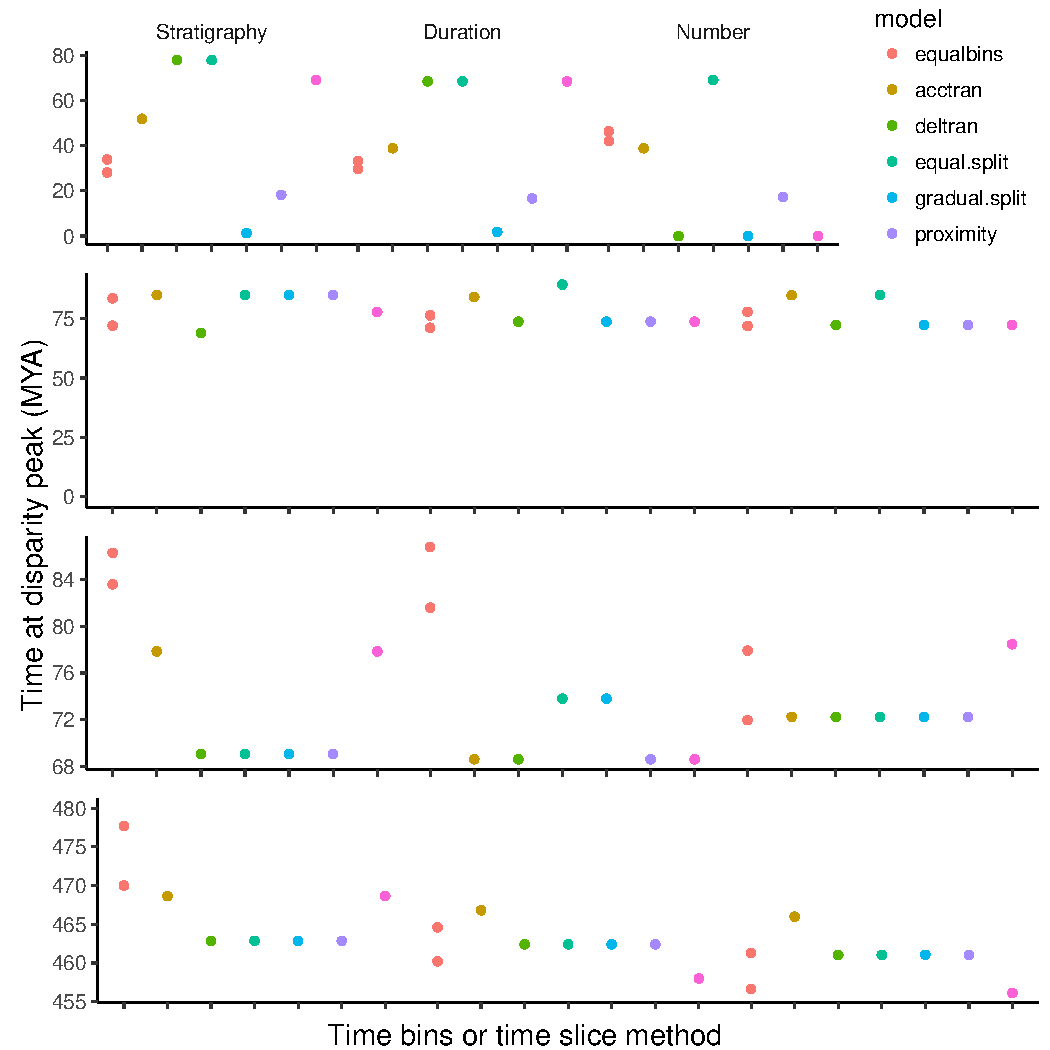
\includegraphics[width=1\linewidth, height=1\textheight, keepaspectratio]{figures/fig-peaks-epoch-appendix.pdf}
    \caption[Timing of peak disparity for four example datasets.]
    {Median bootstrapped disparities were calculated using time binning and time-slicing approaches. 
    %Pink points represent time binning methods, green points are time slices with a punctuated model of evolution (specifically the `proximity' method), and blue points are time slices with a gradual model of evolution (specifically the `gradual splits' method). 
    Stratigraphy uses unequal time bins or non-equidistant slices, where the width of the bin, or the interval between slices, is equivalent to stratigraphic epochs. 
    Duration uses equal time bins or equidistant slices, where the width of the bin, or the interval between slices, is the average duration of stratigraphic epochs in the time frame of the dataset. 
    Number uses equal time bins or equidistant slices, where the number of bins, or the number of slices, is the average number of stratigraphic epochs in the time frame of the dataset. 
    For time bins there are two points indicating the maximum and minimum ages of the time bin within which peak disparities appeared.
    The four dataset names are on the first plot for each dataset (Table \ref{table:datasets}).}
    \label{figure:peak2}
  \end{figure}

\begin{figure}[!htbp]
    \centering
    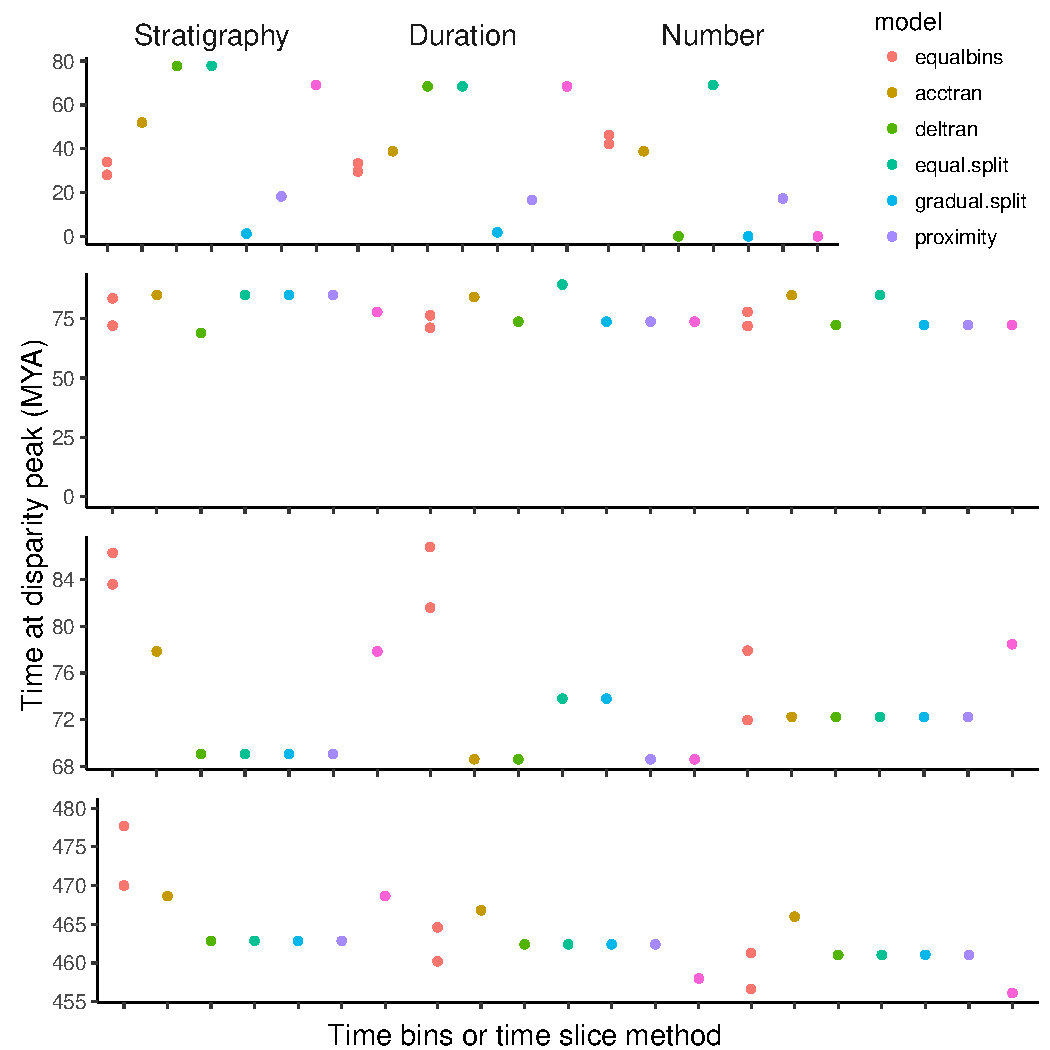
\includegraphics[width=1\linewidth, height=1\textheight, keepaspectratio]{figures/fig-peaks-age-appendix.pdf}
    \caption[Timing of peak disparity for four example datasets.]
    {Median bootstrapped disparities were calculated using time binning and time-slicing approaches. 
    %Pink points represent time binning methods, green points are time slices with a punctuated model of evolution (specifically the `proximity' method), and blue points are time slices with a gradual model of evolution (specifically the `gradual splits' method). 
    Stratigraphy uses unequal time bins or non-equidistant slices, where the width of the bin, or the interval between slices, is equivalent to stratigraphic ages. 
    Duration uses equal time bins or equidistant slices, where the width of the bin, or the interval between slices, is the average duration of stratigraphic ages in the time frame of the dataset. 
    Number uses equal time bins or equidistant slices, where the number of bins, or the number of slices, is the average number of stratigraphic ages in the time frame of the dataset. 
    For time bins there are two points indicating the maximum and minimum ages of the time bin within which peak disparities appeared.
    The four dataset names are on the first plot for each dataset (Table \ref{table:datasets}).}
    \label{figure:peak3}
  \end{figure}

	
\bibliographystyle{palaeo} 
\bibliography{time-refs} 

\end{document}